\section{Web App}

\subsection{Requisiti}
Per poter utilizzare correttamente la web app è necessario disporre di una connessione ad internet e di un browser web che supporti l'estensione Metamask. L'applicazione è stata testata sui seguenti browser:
\begin{itemize}
    \item Google Chrome v112;
    \item Mozilla Firefox v112;
    \item Microsoft Edge v112.
\end{itemize}
L'unico tra i principali browser che non supporta Metamask è Safari, pertanto non è possibile utilizzare la web app su tale browser.

\subsubsection{MetaMask}
Per poter utilizzare la web app è necessaria un'installazione funzionante dell'estensione MetaMask per il browser web.

MetaMask è un portafoglio digitales che permette di interagire con la blockchain Ethereum e con gli smart contract eseguiti su di essa, offrendo la possibilità di effettuare transazioni con diverse criptovalute.

Per le istruzioni di installazione e configurazione di MetaMask si rimanda alla \href{https://support.metamask.io/hc/en-us/articles/360015489531-Getting-started-with-MetaMask}{documentazione ufficiale}.

\subsection{Funzionalità}

\subsubsection{Checkout}
Nella versione finale del prodotto, il checkout sarà integrato direttamente nel sito web del commerciante, e dati quali indirizzo e prezzo da pagare non saranno modificabili dall'utente.

Per motivi di test, è stato implementato un checkout di prova, accessibile inserendo nell'URL indirizzo del destinatario e quantità di ETH da inviare. Se, per esempio, la web app fosse hostata su \path{https://trustify.com} e si volessero inviare 0.1 ETH all'indirizzo \texttt{0x1234567890123456789012345678901234567890}, sarebbe sufficiente accedere all'URL \path{https://trustify.com/checkout/0x1234567890123456789012345678901234567890/0.1}.

Cliccando sul bottone "Paga con Trustify", verrà aperta una finestra di Metamask per confermare la transazione, e si sarà reindirizzati all'interno della web app. Una volta confermata, verrà visualizzata una pagina di conferma del pagamento.

\begin{figure}[H]
    \centering
    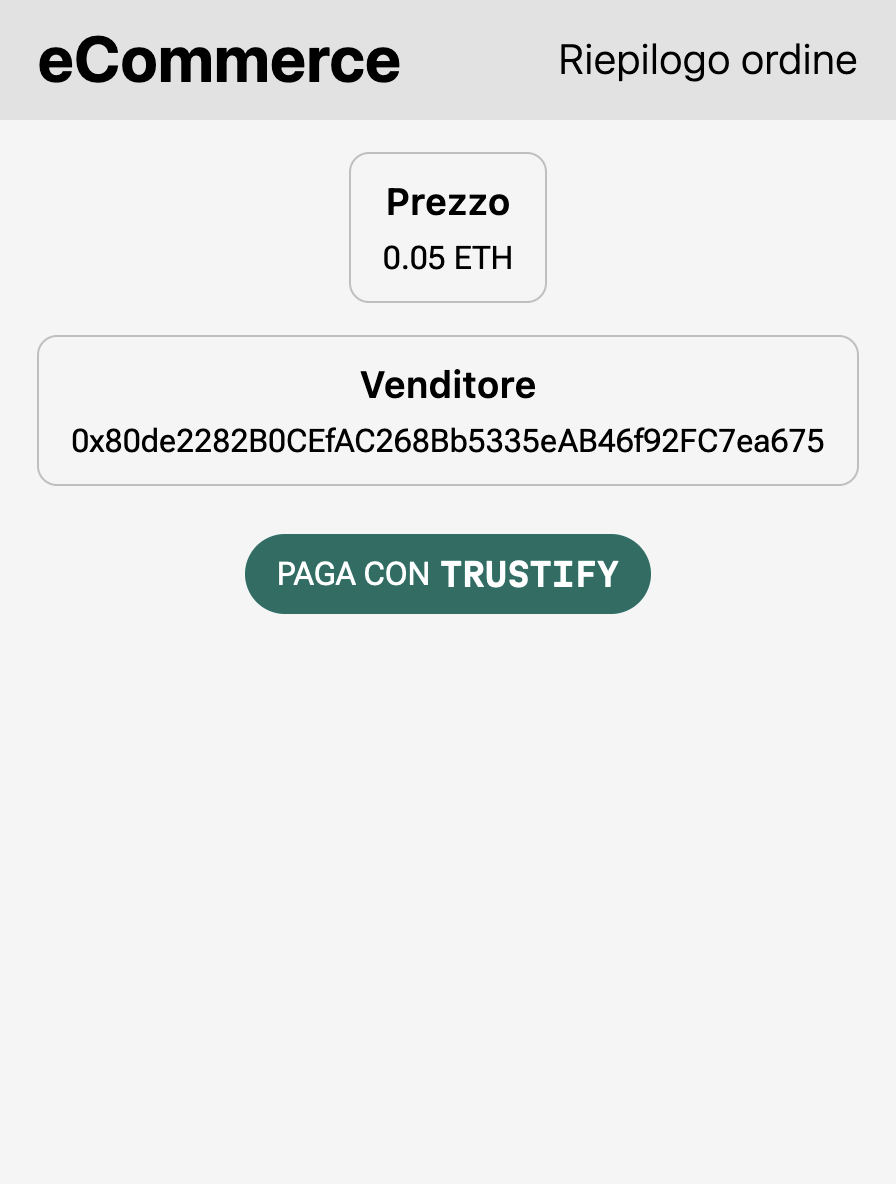
\includegraphics[scale=0.25]{src/img/checkout.png}
    \caption{Pagina di checkout fittizia}
\end{figure}

\subsubsection{Login/Account}

\subsubsection{Pagamenti da recensire}

\subsubsection{Recensioni rilasciate}

\subsubsection{Recensioni ricevute}

\subsubsection{Ricerca recensioni}